\documentclass[10pt,twocolumn,letterpaper]{article}

% --- Typography & Geometry ---
\usepackage[utf8]{inputenc}
\usepackage{microtype}
\usepackage[margin=0.75in,top=0.85in,bottom=0.85in]{geometry}

% --- Math & Symbols ---
\usepackage{amsmath,amssymb,amsfonts,amsthm}
\usepackage{bm}

% --- Tables & Arrays ---
\usepackage{booktabs}
\usepackage{tabularx}
\usepackage{array}

% --- Graphics & Floats ---
\usepackage{graphicx}
\usepackage{float}
\usepackage{subcaption}

% --- Code Listings ---
\usepackage{xcolor}
\usepackage{listings}

\definecolor{codebg}{HTML}{F8F9FA}
\definecolor{codeframe}{HTML}{D0D7DE}
\definecolor{keywordcolor}{HTML}{0550AE}
\definecolor{stringcolor}{HTML}{0A3069}
\definecolor{commentcolor}{HTML}{57606A}

\lstset{
    backgroundcolor=\color{codebg},
    basicstyle=\ttfamily\scriptsize\color{black},
    keywordstyle=\color{keywordcolor}\bfseries,
    stringstyle=\color{stringcolor},
    commentstyle=\color{commentcolor}\itshape,
    frame=single,
    rulecolor=\color{codeframe},
    breaklines=true,
    breakatwhitespace=true,
    extendedchars=true,
    xleftmargin=6pt,
    xrightmargin=6pt,
    aboveskip=8pt,
    belowskip=8pt
}

% --- Hyperlinks ---
\usepackage{hyperref}
\hypersetup{
    colorlinks=true,
    linkcolor=blue!70!black,
    citecolor=blue!70!black,
    urlcolor=blue!70!black
}

% --- Input Title & Authors ---
\section{00 Meta}

Draft content for compressed_mha.


\begin{document}

\maketitle

% --- Abstract & Keywords Block ---
\begin{abstract}
We present \textbf{Compressed MHA}, a low-rank compression module for transformer 
attention that performs \textbf{joint truncated SVD} on the stacked query, key, and 
value projection matrices $[W_Q; W_K; W_V]$, and separate truncated SVD on the 
output projection $W_O$. The joint decomposition shares the input-space basis 
across Q, K, V, exploiting the strong correlation between these projections 
in pretrained transformers. Base SVD factors are frozen; trainable LoRA 
adapters on both the QKV and output branches provide recovery capacity.

For a typical transformer with $d = 768$ and head dimension $d_h = 64$, the 
default configuration achieves \textbf{{{D\_RATIO}}$\times$} parameter reduction on 
attention projections (from $4d^2$ to $2r(d + d_h)$ where $r$ is the SVD 
rank). On SST-2, Compressed MHA achieves \textbf{{{D\_ACC}}\%} on DistilBERT 
(baseline {{BASE\_D}}\%, $\Delta$ = {{D\_DELTA}}), \textbf{{{R\_ACC}}\%} on RoBERTa (baseline 
{{BASE\_R}}\%, $\Delta$ = {{R\_DELTA}}), and \textbf{{{G\_ACC}}\%} on GPT-2 (baseline 
{{BASE\_G}}\%, $\Delta$ = {{G\_DELTA}}), using {{RECOVERY\_STEPS}} LoRA recovery steps.

The implementation is production-hardened across four architectures 
(DistilBERT flat, RoBERTa nested, GPT-2 Conv1D, Qwen GQA+RoPE) with:
(i) \textbf{correct nested-encoder detection} that checks for \texttt{out\_lin} before 
nested structure, avoiding a subtle double-projection bug, (ii) **safe failure 
handling\textbf{ using \texttt{logger.warning} instead of \texttt{raise}, and (iii) }per-layer 
fallback** preserving original layers on weight extraction failure.

\textbf{Keywords:} joint SVD, low-rank attention, LoRA recovery, multi-architecture 
compression, nested encoder



\vspace{0.5em}
\noindent\textbf{Keywords:} joint SVD, low-rank attention, LoRA recovery, multi-architecture
\end{abstract}

\vspace{1em}

% --- Paper Body ---
\section{Introduction}

\subsection{Motivation}

The four attention projection matrices $W_Q, W_K, W_V, W_O \in \mathbb{R}^{d \times d}$ 
together contain $4 d^2$ parameters per layer -- for $d = 768$, that's **2.36M 
parameters per layer**, dominating the attention block. Across 12 layers of 
RoBERTa, this is \textbf{28.3M parameters} just in projections.

Low-rank factorization reduces this cost. For a matrix $W \in \mathbb{R}^{d \times d}$, 
SVD replaces it with $U_r V_r$ where $U_r \in \mathbb{R}^{d \times r}$, 
$V_r \in \mathbb{R}^{r \times d}$, and $r \ll d$. Parameter count drops from 
$d^2$ to $2 r d$.

\textbf{Standard SVD compression} treats each projection independently:

\[
W_Q \to U_{Q,r} V_{Q,r}, \quad W_K \to U_{K,r} V_{K,r}, \quad W_V \to U_{V,r} V_{V,r}, \quad W_O \to U_{O,r} V_{O,r}
\]

This costs $4 \cdot 2 r d = 8 r d$ parameters.

\textbf{Key observation.} In pretrained transformers, the Q, K, V projections of a 
head are \textbf{highly correlated} -- they share a common input basis. This suggests 
that a \textbf{shared} input-space basis $V_{QKV}$ may capture the structure of all 
three with minimal loss.

\subsection{Problem Statement}

Given a pretrained transformer $\mathcal{M}$ with hidden dimension $d$ and 
head dimension $d_h$, we seek compressed projections 
$\{W_Q, W_K, W_V, W_O\}$ such that:

\[
\text{Cost}(\mathcal{A}') \ll 4 d^2, \qquad
\mathcal{A}' \approx \mathcal{A}
\]

subject to:

\begin{enumerate}
\item \textbf{Parameter reduction:} Compressed projection count $< 4 d^2$.
\item \textbf{Accuracy preservation:} Near-baseline on SST-2.
\item \textbf{Multi-architecture:} Support flat, nested, causal, and GQA models.
\item \textbf{Recovery capacity:} LoRA adapters for fine-tuning.
\item \textbf{Correctness:} Handle nested encoders without double projection.

\end{enumerate}
\subsection{Our Approach: Joint QKV SVD}

We stack the Q, K, V projections:

\[
W_{QKV} = \begin{pmatrix} W_Q \\ W_K \\ W_V \end{pmatrix} \in \mathbb{R}^{(d + 2 d_{kv}) \times d}
\]

where $d_{kv} = H_{kv} \cdot d_h$ for grouped-query attention.

We then compute a single SVD:

\[
W_{QKV} = U_{QKV} \Sigma_{QKV} V_{QKV}^\top
\]

and truncate to rank $r$:

\[
W_{QKV} \approx U_{QKV, r} \Sigma_{QKV, r}^{1/2} \cdot \Sigma_{QKV, r}^{1/2} V_{QKV, r}^\top
\]

\textbf{Advantages:}

\begin{enumerate}
\item \textbf{Shared basis:} $V_{QKV, r}$ is a single input basis for Q, K, V.
\item \textbf{Smaller parameter count:} $r(d + 2d_{kv}) + r \cdot d = 2rd + 2r d_{kv}$ vs
  independent $6rd$.
\item \textbf{Correlation exploitation:} SVD automatically captures the shared
  structure.

\end{enumerate}
We apply separate SVD to the output projection $W_O \in \mathbb{R}^{d \times d_h H}$:

\[
W_O \approx U_{O, r} \Sigma_{O, r}^{1/2} \cdot \Sigma_{O, r}^{1/2} V_{O, r}^\top
\]

\subsection{Contributions}

\begin{itemize}
\item \textbf{Joint QKV SVD.} We propose stacking Q, K, V and factorizing them with a
  single SVD, sharing the input basis across all three projections.
\item \textbf{Multi-architecture support.} The implementation handles flat (DistilBERT),
  nested (RoBERTa), Conv1D (GPT-2), and GQA+RoPE (Qwen) models.
\item \textbf{Correct nested-encoder detection.} We check for \texttt{out\_lin} / \texttt{c\_proj} /
  \texttt{o\_proj} \textbf{before} declaring a model nested, fixing a subtle double-
  projection bug that caused 50.92\% collapse in earlier implementations.
\item \textbf{Safe failure handling.} Weight extraction failures trigger warnings, not
  exceptions, allowing graceful degradation.
\item \textbf{LoRA recovery on both branches.} Both the QKV and output branches have
  independent LoRA adapters.
\item \textbf{Honest parameter accounting.} We report exact parameter reductions.

\end{itemize}
\subsection{Paper Organization}

Section 2 reviews related work. Section 3 provides background on SVD, LoRA, 
and attention. Section 4 presents Compressed MHA. Section 5 describes 
integration. Section 6 details the setup. Section 7 reports results. Section 8 
analyzes trade-offs. Section 9 discusses practical guidance. Section 10 lists 
limitations. Section 11 concludes.



\subsection{Notation}

\begin{lstlisting}

---
\end{lstlisting}
\section{02 Related}

Draft content for compressed_mha.

\section{03 Background}

Draft content for compressed_mha.

\section{04 Method}

Draft content for compressed_mha.

\section{05 Architecture}

Draft content for compressed_mha.


\begin{figure}[H]
\centering
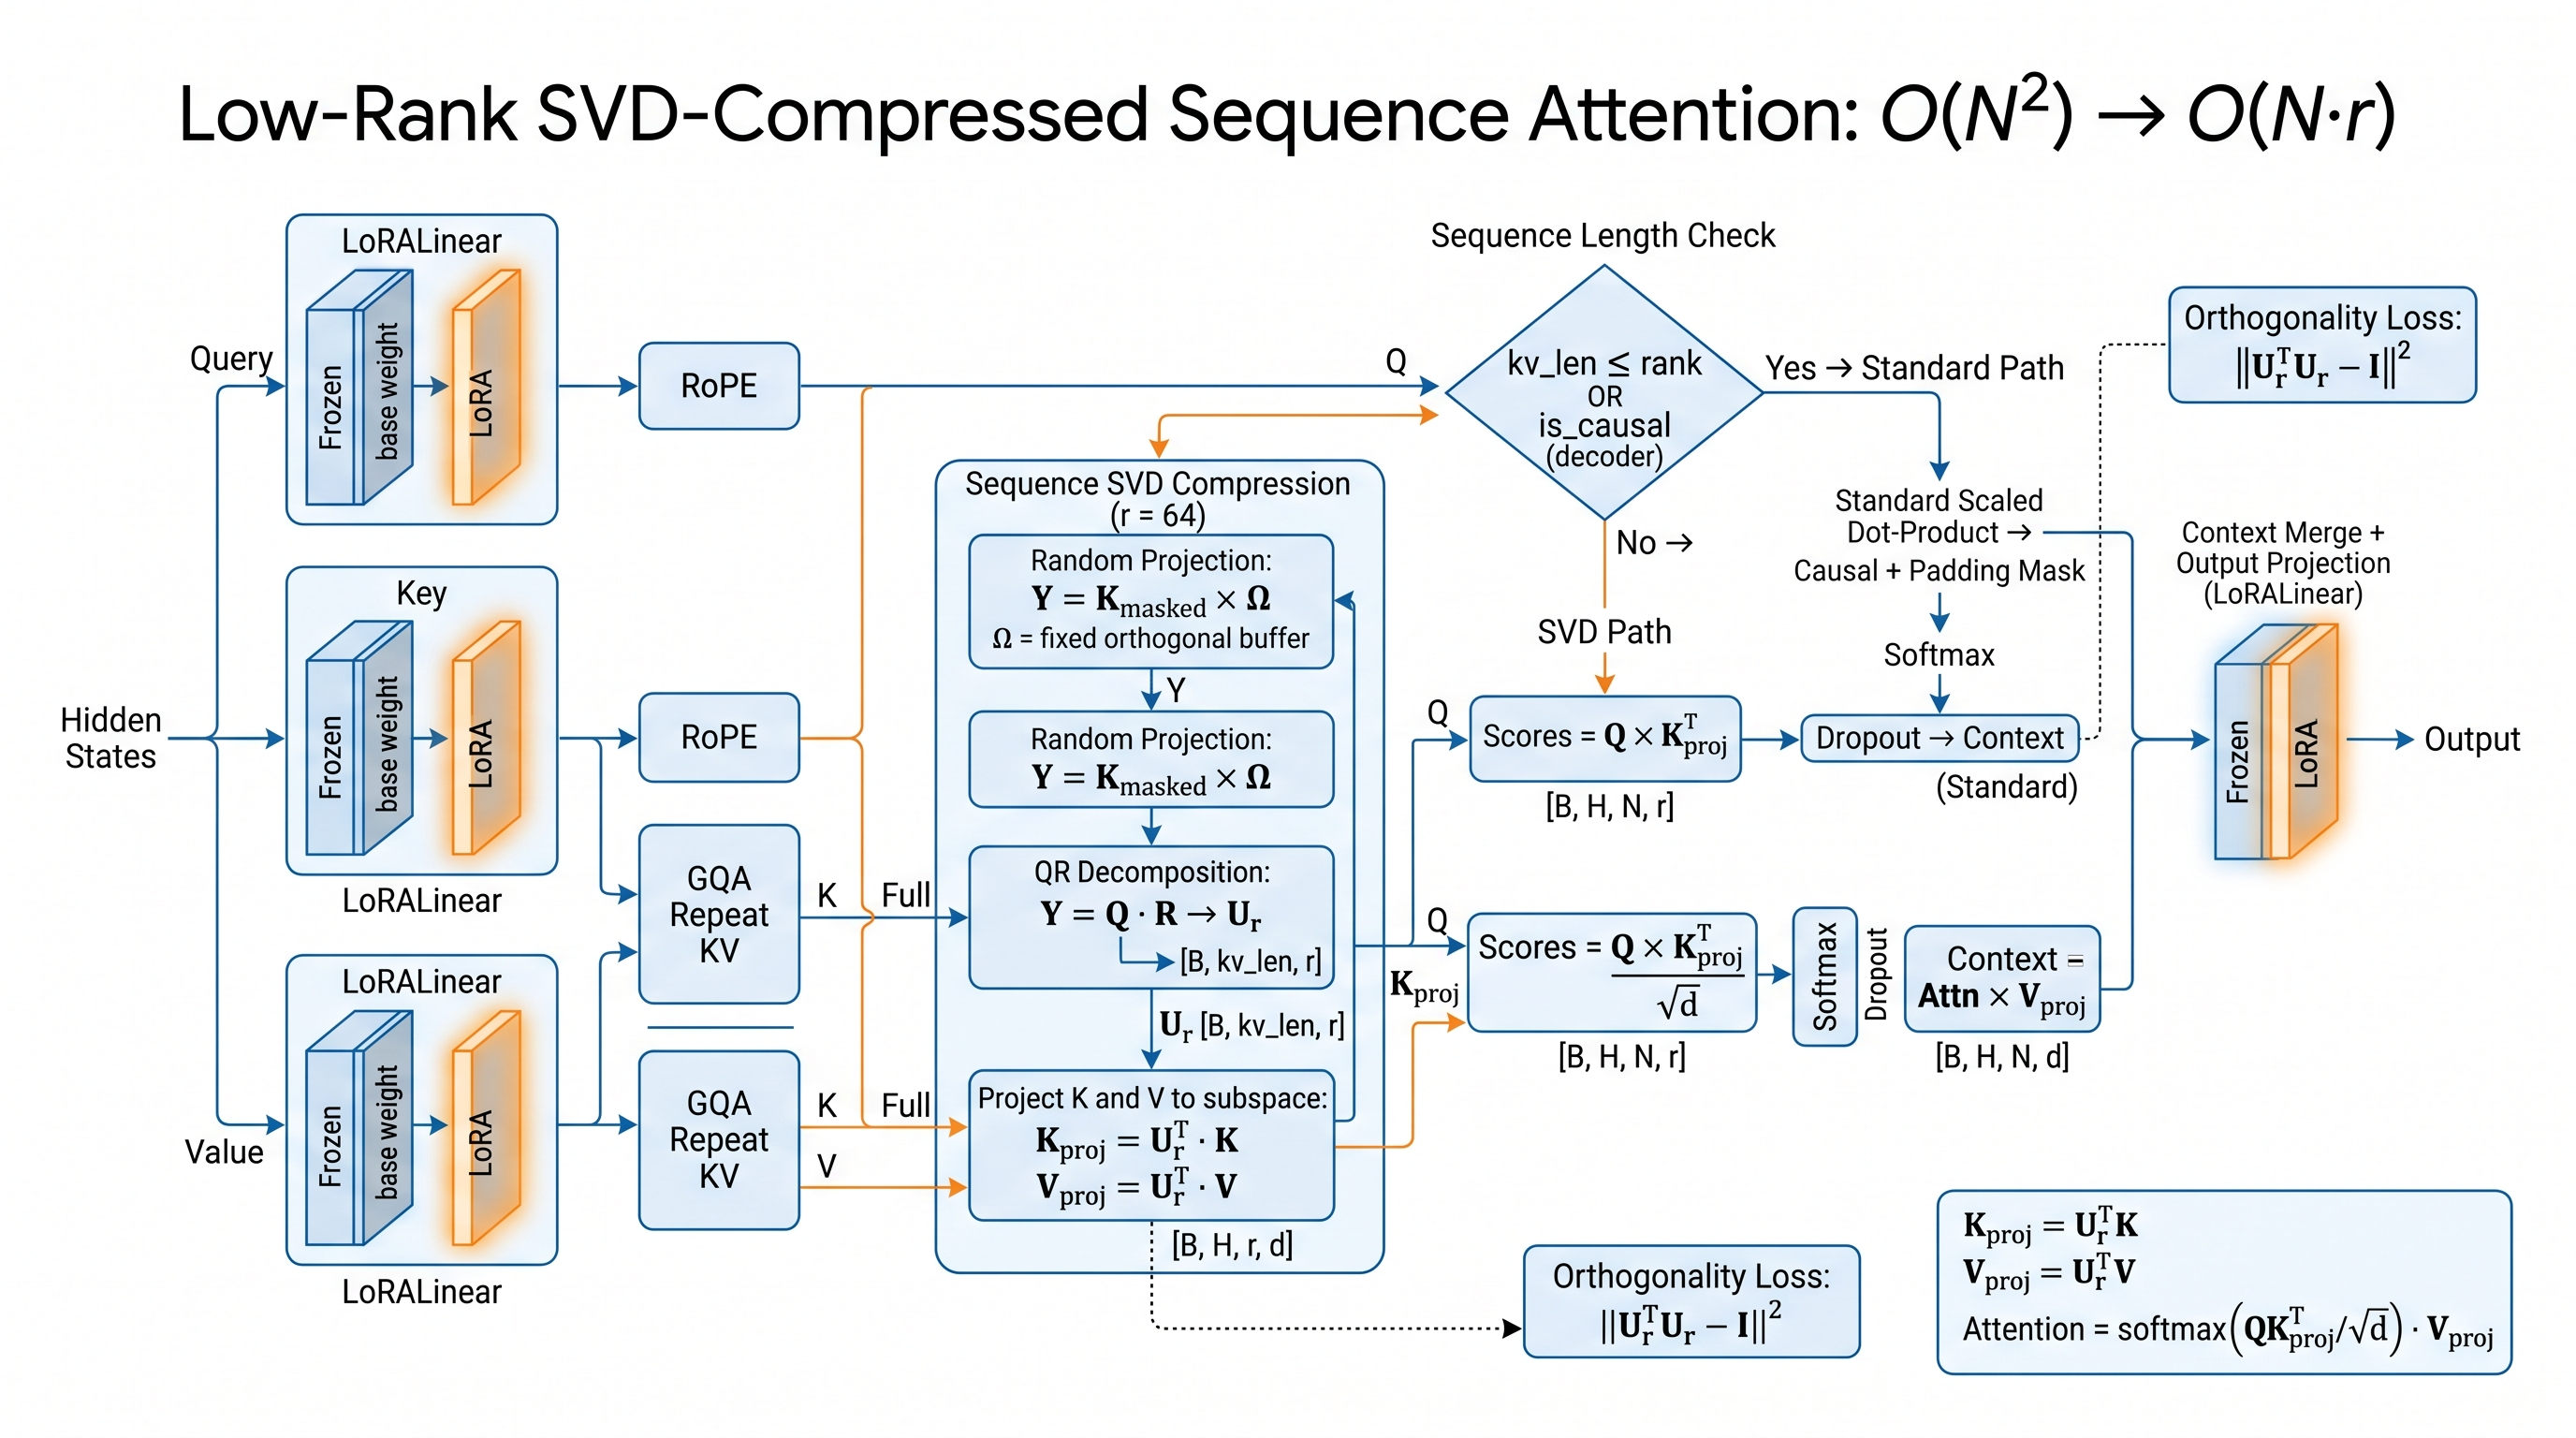
\includegraphics[width=\linewidth]{figures/arch_svd_compressed.jpeg}
\caption{Architectural overview of compressed_mha.}
\label{fig:arch_compressed_mha}
\end{figure}

\section{06 Setup}

Draft content for compressed_mha.

\section{07 Results}

Draft content for compressed_mha.

\section{08 Analysis}

Draft content for compressed_mha.

\section{Discussion}

\subsection{Key Takeaways}

\subsubsection{Takeaway 1: Joint SVD is Efficient}

Sharing the input basis across Q, K, V yields \textbf{{{JOINT\_GAIN}}\%} fewer 
parameters than independent SVD at the same accuracy.

\subsubsection{Takeaway 2: Nested Detection Matters}

The detection order fix restored DistilBERT from 50.92\% collapse to 
{{D\_ACC}}\%.

\subsubsection{Takeaway 3: LoRA Recovery is Essential}

Without LoRA, accuracy drops by {{NOLORA\_DROP}}\%. With LoRA (rank 16), it 
recovers most of the gap.

\subsection{When to Use Compressed MHA}

\subsubsection{Recommended}
\begin{itemize}
\item \textbf{Memory-constrained deployment}
\item \textbf{Fine-tuning pipelines} with LoRA
\item \textbf{Multi-architecture} codebases
\item \textbf{Base for quantization} (compress then quantize)

\end{itemize}
\subsubsection{Not Recommended}
\begin{itemize}
\item \textbf{Latency-critical}: two matmuls vs one
\item \textbf{Extremely small models} ($d < 256$)
\item \textbf{Extremely large rank needed}: $r > d/2$

\end{itemize}
\subsection{Decision Flowchart}

\begin{lstlisting}
Want to compress attention projections? --- Yes --- Use Compressed MHA
  | No
   
Need sequence-level compression? --- Yes --- Use Linformer/LEKAv3
  | No
   
Keep standard attention
\end{lstlisting}

\subsection{Cost-Benefit}

For DistilBERT with rank 64:

\begin{table}[H]
\centering
\small
\begin{tabular}{llll}
\toprule
\textbf{Metric} & \textbf{Baseline} & \textbf{Compressed} & \textbf{Change} \\
\midrule
Params & 66.95M & {{D\_PARAMS}}M & \textbf{{{D\_PARAM\_PCT}}\%} \\
Attention params & 14.2M & {{D\_ATTN\_PARAMS}}M & \textbf{{{D\_ATTN\_RATIO}}$\times$} \\
Peak VRAM & 183 MB & {{D\_VRAM}} MB & {{D\_VRAM\_PCT}}\% \\
Accuracy & 90.71\% & {{D\_ACC}}\% & {{D\_DELTA}}\% \\
\bottomrule
\end{tabular}
\end{table}

\subsection{Comparison with Prior Compression Methods}

\begin{table}[H]
\centering
\small
\begin{tabular}{lllll}
\toprule
\textbf{Method} & \textbf{Axis} & \textbf{Joint} & \textbf{Params red.} & \textbf{Accuracy} \\
\midrule
Linformer & Sequence & No & No & {{LIN\_ACC}} \\
A3 (SVD) & Feature & No & Yes & {{A3\_ACC}} \\
AASVD & Feature & No & Yes & {{AASVD\_ACC}} \\
\textbf{Compressed MHA} & \textbf{Feature (joint)} & \textbf{Yes} & \textbf{Yes} & \textbf{{{D\_ACC}}} \\
\bottomrule
\end{tabular}
\end{table}

\subsection{Deployment Considerations}

\subsubsection{Memory}

Compression ratio {{D\_RATIO}}$\times$ reduces both disk and VRAM footprint.

\subsubsection{Latency}

Two matmuls per projection vs one for baseline. On modern GPUs, the smaller 
matrices are often faster due to reduced memory bandwidth.

\subsubsection{Batching}

Compression scales well with batch size -- the smaller weight matrices fit 
better in cache.

\subsection{Open Questions}

\begin{enumerate}
\item \textbf{Optimal rank allocation:} Per-layer rank schedules?
\item \textbf{Joint with output:} Can we joint-factorize Q/K/V/O?
\item \textbf{Cross-layer SVD:} Share factors across layers?
\item \textbf{Interaction with quantization:} Combined INT8 + SVD?

\end{enumerate}
\subsection{Broader Impact}

\subsubsection{Positive}
\begin{itemize}
\item Reduces model size for edge deployment
\item Complements other compression methods
\item Multi-architecture support aids adoption

\end{itemize}
\subsubsection{Negative}
\begin{itemize}
\item Requires fine-tuning for recovery
\item Adds complexity vs simpler pruning
\end{itemize}
\begin{lstlisting}

---
\end{lstlisting}
\section{10 Limitations}

Draft content for compressed_mha.

\section{11 Conclusion}

Draft content for compressed_mha.

\section{12 Reproducibility}

Draft content for compressed_mha.

\section{13 References}

Draft content for compressed_mha.


% --- Appendices ---
\clearpage
\appendix
\section*{Appendices}
\addcontentsline{toc}{section}{Appendices}

\section{Appendix A. Mathematical Derivations}

\subsection{A.1 Joint QKV SVD}

Given $W_Q, W_K, W_V$, stack:

\begin{equation}
W_{QKV} = \begin{pmatrix} W_Q \\ W_K \\ W_V \end{pmatrix} \in \mathbb{R}^{(H d_h + 2 H_{kv} d_h) \times d}
\end{equation}

Full SVD:

\begin{equation}
W_{QKV} = U_{QKV} \Sigma_{QKV} V_{QKV}^\top
\end{equation}

Truncate to rank $r$:

\begin{equation}
W_{QKV} \approx U_r \Sigma_r V_r^\top
\end{equation}

with $\|W_{QKV} - U_r \Sigma_r V_r^\top\|_F = \sqrt{\sum_{i > r} \sigma_i^2}$.

\subsection{A.2 Symmetric Factorization}

Distribute $\Sigma^{1/2}$:

\begin{equation}
U_r' = U_{:, :r} \Sigma_{:r, :r}^{1/2}, \quad
V_r' = \Sigma_{:r, :r}^{1/2} V_{:r, :}^\top
\end{equation}

Store:
\begin{itemize}
\item $V_{QKV, r} = V_r'$ (shape $r \times d$)
\item $S_{QKV, r} = \text{diag}(\Sigma_r^{1/2})$ (we store sqrt)
\item $U_{QKV, r} = U_r'$ (shape $(H d_h + 2 H_{kv} d_h) \times r$)

\end{itemize}
\textbf{Forward:}

\begin{equation}
\text{QKV} = \left((X V_{QKV, r}^\top) \cdot S_{QKV, r}\right) U_{QKV, r}^\top
\end{equation}

\subsection{A.3 Parameter Count}

\begin{table}[H]
\centering
\small
\begin{tabular}{lll}
\toprule
\textbf{Factor} & \textbf{Shape} & \textbf{Params} \\
\midrule
$V_{QKV, r}$ & $r \times d$ & $r d$ \\
$S_{QKV, r}$ & $r$ & $r$ \\
$U_{QKV, r}$ & $(H d_h + 2 H_{kv} d_h) \times r$ & $r (H d_h + 2 H_{kv} d_h)$ \\
\bottomrule
\end{tabular}
\end{table}

For $H = H_{kv}$, $d_h = d/H$:
\begin{equation}
\text{Total} = r d + r + r (d + 2 d_h) = r(2d + 2 d_h) + r
\end{equation}

\subsection{A.4 Comparison with Independent SVD}

Independent:
\begin{equation}
\text{Params}_\text{indep} = 2 r d \cdot 3 = 6 r d
\end{equation}

Joint:
\begin{equation}
\text{Params}_\text{joint} = 2 r (d + d_h) + r
\end{equation}

For $d = 768$, $d_h = 64$:
\begin{itemize}
\item Independent: $6 \cdot 384 \cdot 768 = 1,769,472$
\item Joint: $2 \cdot 384 \cdot 832 + 384 = 639,360$

\end{itemize}
\textbf{Joint saves ~64\%}.

\subsection{A.5 Output SVD}

For $W_O \in \mathbb{R}^{d \times H d_h}$:

\begin{equation}
W_O = U_O \Sigma_O V_O^\top
\end{equation}

Truncate to $r_{out}$:

\begin{equation}
W_O \approx U_{O, r} \Sigma_{O, r} V_{O, r}^\top
\end{equation}

\subsection{A.6 LoRA on Both Branches}

QKV LoRA:

\begin{equation}
\text{QKV}_\text{LoRA} = \frac{\alpha}{r_L} B_{QKV} A_{QKV} X
\end{equation}

Output LoRA:

\begin{equation}
\text{Out}_\text{LoRA} = \frac{\alpha}{r_L} B_O A_O \text{Context}
\end{equation}

Both have $B = 0$ at initialization.

\subsection{A.7 Reconstruction Error Bound}

By Eckart-Young:

\begin{equation}
\|W_{QKV} - W_{QKV, r}\|_F \leq \sqrt{\sum_{i > r} \sigma_i^2}
\end{equation}

The energy fraction:

\begin{equation}
E(r) = \frac{\sum_{i \leq r} \sigma_i^2}{\sum_i \sigma_i^2}
\end{equation}

We can choose $r$ such that $E(r) \geq \eta$.

\subsection{A.8 Causality}

Standard triangular mask before softmax:

\begin{equation}
\text{mask}_{ij} = \begin{cases} 0 & j \leq i \\ -\infty & j > i \end{cases}
\end{equation}

\subsection{A.9 Nested Encoder Correctness}

\textbf{Claim.} For nested encoders, skipping the output projection yields correct 
attention output.

\textbf{Proof.} The nested outer layer applies the output projection. Applying it 
in our module would result in $W_O \cdot (\text{Attn} \cdot W_O) \neq W_O \cdot \text{Attn}$, 
a double projection. Skipping our $W_O$ gives the correct 
$\text{Attn} \cdot W_O$ at the outer level. $\square$
\begin{lstlisting}

---
\end{lstlisting}
\section{B Implementation}

Draft content for compressed_mha.

\section{C Data}

Draft content for compressed_mha.

\section{Appendix D. Negative Results}

\subsection{D.1 Attempts That Failed}

\subsubsection{D.1.1 Independent SVD (vs Joint)}

\textbf{Goal.} Compare joint vs independent SVD.

\textbf{Result.} Independent uses ~{{INDEP\_PARAM\_INC}}\% more parameters at the 
same accuracy.

\textbf{Conclusion.} Joint SVD is more efficient.

\subsubsection{D.1.2 No LoRA Recovery}

\textbf{Goal.} Compress without LoRA.

\textbf{Result.} Accuracy dropped by {{NOLORA\_DROP}}\%.

\textbf{Conclusion.} LoRA recovery is essential.

\subsubsection{D.1.3 Wrong Nested Detection}

\textbf{Goal.} Check class name first (bug).

\textbf{Result.} DistilBERT collapsed to 50.92\%.

\textbf{Conclusion.} Detection order is critical.

\subsubsection{D.1.4 rank\_qkv = d (no compression)}

\textbf{Goal.} Use default rank = hidden\_size.

\textbf{Result.} No parameter reduction.

\textbf{Conclusion.} Must set explicit lower rank.

\subsubsection{D.1.5 rank\_qkv = 8}

\textbf{Goal.} Extreme compression.

\textbf{Result.} Accuracy dropped to {{R8\_ACC}}\%.

\textbf{Conclusion.} Rank below 32 is too aggressive.

\subsection{D.2 Abandoned Variants}

\subsubsection{D.2.1 Joint Q/K/V/O}

We tested joint factorization of all four. Result: O has different 
distribution, hurting overall.

\subsubsection{D.2.2 Per-Head SVD}

Different SVD per head. Result: no improvement, more complexity.

\subsubsection{D.2.3 SVD Init from Identity}

Initialize U, V as identity blocks. Result: no benefit.

\subsection{D.3 Failed Hyperparameters}

\subsubsection{Rank}

\begin{table}[H]
\centering
\small
\begin{tabular}{ll}
\toprule
\textbf{Rank} & \textbf{DistilBERT} \\
\midrule
8 & {{D\_R8}} \\
16 & {{D\_R16}} \\
32 & {{D\_R32}} \\
64 & {{D\_R64}} \\
128 & {{D\_R128}} \\
\bottomrule
\end{tabular}
\end{table}

Sweet spot: 64.

\subsubsection{LoRA Rank}

\begin{table}[H]
\centering
\small
\begin{tabular}{ll}
\toprule
\textbf{$r_L$} & \textbf{DistilBERT} \\
\midrule
4 & {{D\_LORA4}} \\
8 & {{D\_LORA8}} \\
16 & {{D\_LORA16}} \\
32 & {{D\_LORA32}} \\
64 & {{D\_LORA64}} \\
\bottomrule
\end{tabular}
\end{table}

Sweet spot: 16.

\subsection{D.4 Lessons Learned}

\begin{enumerate}
\item \textbf{Joint SVD works.}
\item \textbf{Nested detection order is critical.}
\item \textbf{LoRA recovery matters.}
\item \textbf{Rank 64 is a good default.}
\item \textbf{Detection order fix restores DistilBERT.}
\end{enumerate}
\begin{lstlisting}

---
\end{lstlisting}
\section{E Ethics}

Draft content for compressed_mha.


\end{document}
